\clearpage
\section{Результаты вычислительных экспериментов}
	Архитектуры, описанные в пункте 1.4.3, а так же модификация процедуры обучения, описанная в 1.4.4 были реализованы в виде комплекса программ на языке Python с помощью библиотеки для глубокого обучения PyTorch. Использованные версии программных пакетов указаны в Приложении 1. Обучение проводилось на наборе данных Berea.
	\subsection{Набор данных Berea}
		Исходные данные - изображение компьютерной томографии песчаника, объёмом $400^3$ вокселей, бинарно сегментированная на породу и поры, в формате TIFF. Для обучения сетей из этого кубика был вырезан набор кубиков размером $64^3$ вокселей, с перекрытием в 16 вокселей, они и представили собой обучающую выборку. Оригинальный образец размером $400^3$ вокселей представлен на (Рис. \ref{5-full-berea}). Некоторые примеры из получившейся обучающей выборки представлены в (Таб. \ref{5-berea64}).
		
		\begin{figure}[h!]
			\centering{\includegraphics[width=0.6\linewidth]{5-results/berea/original}}
			\caption{Оригинальный образец}
			\label{5-full-berea}
		\end{figure}
	
		\begin{table}[h!]
			\begin{center}
				\begin{tabular}{p{5cm} p{5cm} p{5cm}}
					\toprule
					\includegraphics[width=0.9\linewidth]{5-results/berea/berea_1}
					&
					\includegraphics[width=0.9\linewidth]{5-results/berea/berea_2}
					&
					\includegraphics[width=0.9\linewidth]{5-results/berea/berea_3}
					\\
					\includegraphics[width=0.9\linewidth]{5-results/berea/berea_4}
					&
					\includegraphics[width=0.9\linewidth]{5-results/berea/berea_5}
					&
					\includegraphics[width=0.9\linewidth]{5-results/berea/berea_6}
					\\
					\bottomrule
				\end{tabular}
				\caption{Примеры из обучающей выборки}
				\label{5-berea64}
			\end{center}
		\end{table}
	\subsection{Обучение нейросети}
		Было проведено обучение нейросети со следующими параметрами (число сверточных фильтров указано для первого слоя):
		\begin{table}[h!]
			\begin{center}
				\begin{tabular}{|c|c|c|c|}
					\hline
					Число фильтров G, D & Размерность z & Размер пакета & Начальный LR \\
					\hline
					64, 32 & 512 & 64 & 2e-4 \\
					\hline
				\end{tabular}
				\caption{Гиперпараметры нейросети и процесса обучения}
			\end{center}
		\end{table}
		
		Графики функций ошибок сетей генератора и дискриминатора, а также графики сходимостей функционалов Минковского в процессе обучения приведены на (Рис. \ref{loss-plot}, \ref{V-plot}, \ref{S-plot}, \ref{B-plot}, \ref{Xi-plot}).
		
		\begin{figure}[h!]
			\centering{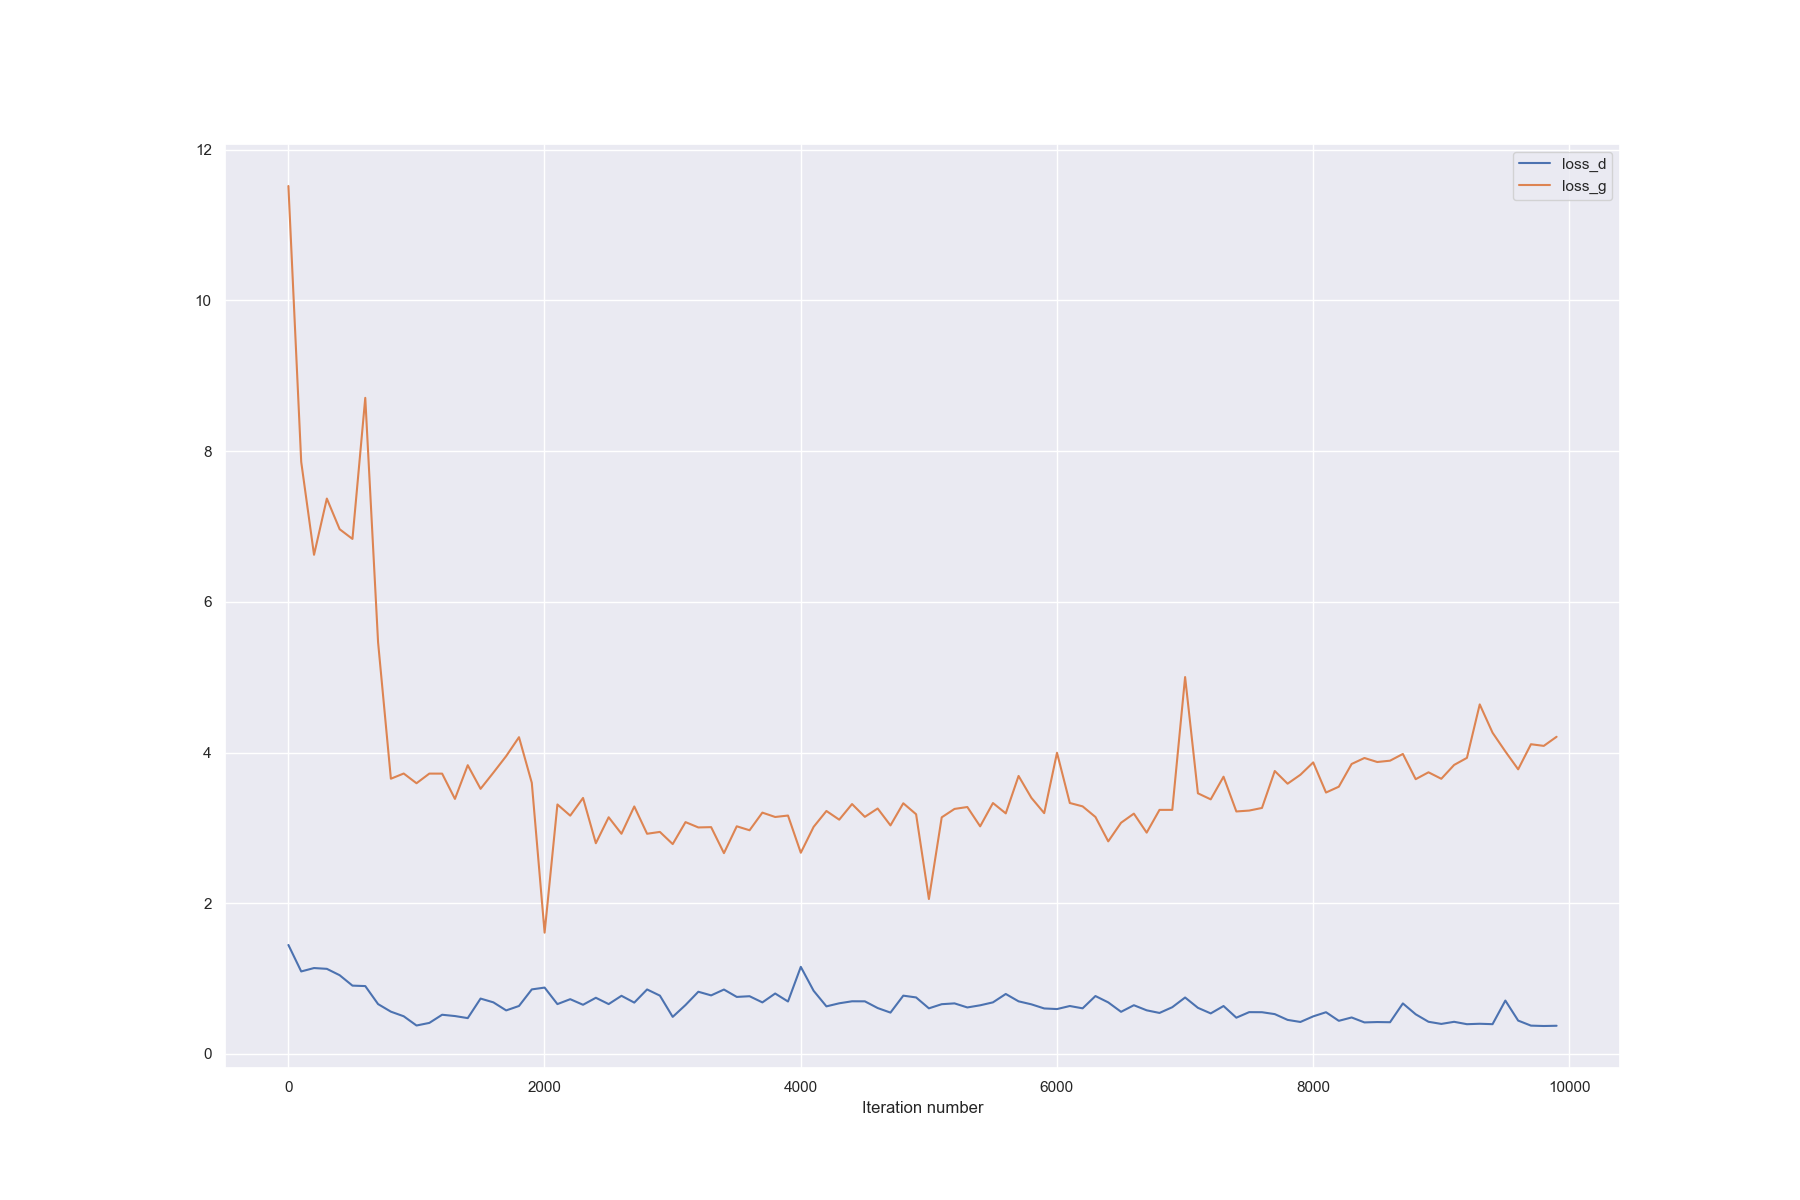
\includegraphics[width=0.95\linewidth]{5-results/experiment/loss_plot}}
			\caption{График функций ошибок сетей дискриминатора и генератора}
			\label{loss-plot}
		\end{figure}
	
		\begin{figure}[h!]
			\centering{\includegraphics[width=0.95\linewidth]{5-results/experiment/minkowski_V_plot}}
			\caption{График сходимости функционала Минковского $V$}
			\label{V-plot}
		\end{figure}
		
		\begin{figure}[h!]
			\centering{\includegraphics[width=0.95\linewidth]{5-results/experiment/minkowski_S_plot}}
			\caption{График сходимости функционала Минковского $S$}
			\label{S-plot}
		\end{figure}
	
		\begin{figure}[h!]
			\centering{\includegraphics[width=0.95\linewidth]{5-results/experiment/minkowski_B_plot}}
			\caption{График сходимости функционала Минковского $B$}
			\label{B-plot}
		\end{figure}
	
		\begin{figure}[h!]
			\centering{\includegraphics[width=0.95\linewidth]{5-results/experiment/minkowski_Xi_plot}}
			\caption{График сходимости функционала Минковского $\xi$}
			\label{Xi-plot}
		\end{figure}	
		
	
	\subsection{Реконструкции размера $64^3$}
		\subsubsection{Примеры синтеза}
	
			Примеры реконструкции размера $64^3$, приведены в (Таб. \ref{5-gen-64}).
			
			\begin{table}[h!]
				\begin{center}
					\begin{tabular}{p{5cm} p{5cm} p{5cm}}
						\toprule
						\includegraphics[width=1\linewidth]{5-results/berea/original}
						&
						\includegraphics[width=1\linewidth]{5-results/berea/original}
						&
						\includegraphics[width=1\linewidth]{5-results/berea/original}
						\\
						\includegraphics[width=1\linewidth]{5-results/berea/original}
						&
						\includegraphics[width=1\linewidth]{5-results/berea/original}
						&
						\includegraphics[width=1\linewidth]{5-results/berea/original}
						\\
						\includegraphics[width=1\linewidth]{5-results/berea/original}
						&
						\includegraphics[width=1\linewidth]{5-results/berea/original}
						&
						\includegraphics[width=1\linewidth]{5-results/berea/original}
						\\
						\bottomrule
					\end{tabular}
					\caption{Примеры реконструкции 64x64x64}
					\label{5-gen-64}
				\end{center}
			\end{table} 
		
		\subsubsection{Анализ реконструкций}
			Было реконструировано 100 образцов размера $64^3$. На основе этого набора были получены распределения интересующих функционалов Минковского. Так же, используя предоставленную\cite{Mosser} сеть, было реконструировано 1000 образцов  того же размера для сравнения распределений функционалов. Графики полученных распределений приведены на (Рис. \ref{5-dist-V}, \ref{5-dist-S}, \ref{5-dist-B}, \ref{5-dist-Xi})
			
			\begin{figure}[h]
				\begin{minipage}[h]{0.49\linewidth}
					\centering{\includegraphics[width=1\linewidth]{5-results/analysis_64/V_exp} \\ Обученная сеть}
				\end{minipage}
				\hfill
				\begin{minipage}[h]{0.49\linewidth}
					\centering{\includegraphics[width=1\linewidth]{5-results/analysis_64/V_paper} \\ Предоставленная\cite{Mosser} сеть}
				\end{minipage}
				\caption{Распределения функционала Минковского $V$}
				\label{5-dist-V}
			\end{figure}
		
			\begin{figure}[h]
				\begin{minipage}[h]{0.49\linewidth}
					\centering{\includegraphics[width=1\linewidth]{5-results/analysis_64/S_exp} \\ Обученная сеть}
				\end{minipage}
				\hfill
				\begin{minipage}[h]{0.49\linewidth}
					\centering{\includegraphics[width=1\linewidth]{5-results/analysis_64/S_paper} \\ Предоставленная\cite{Mosser} сеть}
				\end{minipage}
				\caption{Распределения функционала Минковского $S$}
				\label{5-dist-S}
			\end{figure}
		
			\begin{figure}[h]
				\begin{minipage}[h]{0.49\linewidth}
					\centering{\includegraphics[width=1\linewidth]{5-results/analysis_64/B_exp} \\ Обученная сеть}
				\end{minipage}
				\hfill
				\begin{minipage}[h]{0.49\linewidth}
					\centering{\includegraphics[width=1\linewidth]{5-results/analysis_64/B_paper} \\ Предоставленная\cite{Mosser} сеть}
				\end{minipage}
				\caption{Распределения функционала Минковского $B$}
				\label{5-dist-B}
			\end{figure}
		
			\begin{figure}[h]
				\begin{minipage}[h]{0.49\linewidth}
					\centering{\includegraphics[width=1\linewidth]{5-results/analysis_64/Xi_exp} \\ Обученная сеть}
				\end{minipage}
				\hfill
				\begin{minipage}[h]{0.49\linewidth}
					\centering{\includegraphics[width=1\linewidth]{5-results/analysis_64/Xi_paper} \\ Предоставленная\cite{Mosser} сеть}
				\end{minipage}
				\caption{Распределения функционала Минковского $\xi$}
				\label{5-dist-Xi}
			\end{figure}
			
